
%(BEGIN_QUESTION)
% Copyright 2011, Tony R. Kuphaldt, released under the Creative Commons Attribution License (v 1.0)
% This means you may do almost anything with this work of mine, so long as you give me proper credit

An Allen-Bradley PLC controls the starting and stopping of a conveyor belt, taking inputs from both hard-wired pushbutton switches as well as from an HMI panel connected to the PLC.  This particular system has a problem, though.  The conveyor starts, but the warning siren does not alert before start-up like it is supposed to.  The system is brand-new, and has exhibited this problem from the very first day it was run.  A live-status view of the program seen while the conveyor is running reveals the following:

$$\includegraphics[width=15.5cm]{i03578x01.eps}$$

Based on the information gathered from this live-status view, what do you think is wrong with the system?  Explain your answer.

\underbar{file i03578}
%(END_QUESTION)





%(BEGIN_ANSWER)

{\it Half-credit for fault, half-credit for explanation why.}

\vskip 10pt

The problem is with the ``HMI\_Silence'' bit {\tt B3:0/2}.  The bit has a value of 0, when it should have a value of 1.  Either this is an operator error (unintentionally silencing the alarm) or else there is a problem in the HMI or in the HMI/PLC communications where the data bit from the HMI is not properly arriving at the PLC.

%(END_ANSWER)





%(BEGIN_NOTES)

{\bf This question is intended for exams only and not worksheets!}.

%(END_NOTES)


